\documentclass{article}
\usepackage[letterpaper]{geometry}
\geometry{verbose,tmargin=1in,bmargin=1in,lmargin=1in,rmargin=1in}

\usepackage[utf8]{inputenc}
\usepackage{amsmath}
\usepackage{amssymb}
\usepackage{listings}
\usepackage{graphicx}
\usepackage{enumitem}

\title{CIS 419/519: Homework 2}
\author{Jiatong Sun}
\date{}

\begin{document}
    \maketitle
	Although the solutions are entirely my own, I consulted with the following people and sources while working on this homework: $Junfan Pan$, $Zhuoyu He$, $Yuchen Sun$, $Chang Liu$, $Yihang Xu$, $Yupeng Li$ \\
    $https://machinelearningmastery.com/understand-the-dynamics-of-learning-rate-on-deep-learning-neural-networks/$\\
    $https://en.wikipedia.org/wiki/Learning_rate$\\
    $https://machinelearningmastery.com/how-to-tune-algorithm-parameters-with-scikit-learn/$.
    
    \section{Gradient Descent}
        \begin{enumerate}[label=\alph*.]
            \item % a
            The implication of the learning rate $\alpha_{k}$ is to control how big a step should be taken in the gradient descent direction towards the minimum, where a too small $\alpha_{k}$ may result in a long training time and a too large $\alpha_{k}$ may lead to an overshooting training process.
            
            
            \item % b
            The implications of setting $\alpha_{k}$ as a function of k is to select an adaptive learning rate based on the training process, since the best step to take can vary as the the training goes gradually towards the minimum and a preset constant $\alpha_{k}$ may not work well in the whole process.
        \end{enumerate}
        
       \section{Linear Regression [CIS 519 ONLY]}
       	Since 
       	\begin{equation}
       		y_i=f(\boldsymbol{x_i})+\epsilon_i
       	\end{equation}
       	and
       	\begin{equation}
        	\epsilon_i \sim G(0, \sigma^2)
       	\end{equation}
       	We can know that function $f$ is the linear regression function without error
       	\begin{equation}
       		f(\boldsymbol{x_i})= \theta_0+\sum_{j=1}^{d}\theta_j x_{ij}=\sum_{j=0}^{d}\theta_j x_{ij}, (x_{i0}=1)       
       	\end{equation}
       	or in matrix form
       	\begin{equation}\label{eq:reg}
       		f(\boldsymbol{x_i})=\boldsymbol{x_i}\boldsymbol{\theta}
       	\end{equation}
       	where
       	\begin{equation}
       		\boldsymbol{x_i} = \begin{bmatrix} 
    			1&x_{i1}&\dots&x_{ij}&\dots&x_{id}
    			\end{bmatrix}
    	\end{equation}
    	\begin{equation}
       		\boldsymbol{\theta} = \begin{bmatrix} 
    			\theta_0&\theta_1&\dots&\theta_j&\dots&\theta_d
    			\end{bmatrix}^T
       	\end{equation}
       	From the closed form solution, we can write $\theta$ in the following format
       	\begin{equation}\label{eq:close}
       		\boldsymbol{\theta} = (\boldsymbol{X}^T\boldsymbol{X})^{-1}\boldsymbol{X}^T\boldsymbol{y}
       	\end{equation}
       	where $\boldsymbol{X}$ represents the whole training set and $\boldsymbol{y}$ represents its label
       	\begin{equation}
           	\boldsymbol{X} = \begin{bmatrix} 
    			\boldsymbol{x_1}\\\boldsymbol{x_2}\\\vdots\\\boldsymbol{x_i}\\\vdots\\\boldsymbol{x_n}
    			\end{bmatrix}= \begin{bmatrix} 
    			1&x_{11}&\dots&x_{1j}&\dots&x_{1d}\\
    			1&x_{21}&\dots&x_{2j}&\dots&x_{2d}\\
    			\vdots&\vdots&     &\vdots&     &\vdots\\
    			1&x_{i1}&\dots&x_{ij}&\dots&x_{id}\\
    			\vdots&\vdots&     &\vdots&     &\vdots\\
    			1&x_{n1}&\dots&x_{nj}&\dots&x_{nd}\\
    			\end{bmatrix},
       	\end{equation}
       	\begin{equation}
       		\boldsymbol{y} = \begin{bmatrix} 
    			y_0&y_1&\dots&y_i&\dots&y_n
    			\end{bmatrix}^T
       	\end{equation}
       	Let $\boldsymbol{x}$ be a column vector, which represents \textbf{\emph{the test data set instead of the training data set}}. \\\\
       	From \eqref{eq:reg}, we can write $f(\boldsymbol{x})$ in the following format
       	\begin{equation}
            f(\boldsymbol{x}) = h_{\boldsymbol{\theta}}(\boldsymbol{x})= \boldsymbol{x}\boldsymbol{\theta}
       	\end{equation}
       	where
       	\begin{equation}
           	\boldsymbol{x} = \begin{bmatrix} 
    			\boldsymbol{t_1}\\\boldsymbol{t_2}\\\vdots\\\boldsymbol{t_k}\\\vdots\\\boldsymbol{t_m}
    			\end{bmatrix}= \begin{bmatrix} 
    			1&t_{11}&\dots&t_{1j}&\dots&t_{1d}\\
    			1&t_{21}&\dots&t_{2j}&\dots&t_{2d}\\
    			\vdots&\vdots&     &\vdots&     &\vdots\\
    			1&t_{k1}&\dots&t_{kj}&\dots&t_{kd}\\
    			\vdots&\vdots&     &\vdots&     &\vdots\\
    			1&t_{m1}&\dots&t_{mj}&\dots&t_{md}\\
    			\end{bmatrix},
       	\end{equation}
       	Here, we use $\boldsymbol{t_k}$ and $\boldsymbol{t_m}$ to replace $\boldsymbol{x_i}$ and $\boldsymbol{x_n}$ so we can distinguish the training data and the test data.\\\\
       	From \eqref{eq:reg} and \eqref{eq:close}, we  get
       	\begin{equation}\label{eq:f}
            f(\boldsymbol{x}) = \boldsymbol{x} (\boldsymbol{X}^T\boldsymbol{X})^{-1}\boldsymbol{X}^T\boldsymbol{y}
       	\end{equation}
       	where the dimensions are $\boldsymbol{x}=\boldsymbol{x}_{m\times (d+1)}$, $\boldsymbol{X}=\boldsymbol{X}_{n\times (d+1)}$, $\boldsymbol{y}=\boldsymbol{y}_{n\times1}$\\\\ 
       	So $\boldsymbol{x} (\boldsymbol{X}^T\boldsymbol{X})^{-1}\boldsymbol{X}^T$ has the dimension of $[m\times n]$, or
       	\begin{equation}
       		\boldsymbol{L}_{m\times n}\triangleq\boldsymbol{x} (\boldsymbol{X}^T\boldsymbol{X})^{-1}\boldsymbol{X}^T=
       			\begin{bmatrix} 
       			L_{10}&L_{11}&\dots&L_{1i}&\dots&L_{1n}\\
    			L_{20}&L_{21}&\dots&L_{2i}&\dots&L_{2n}\\
    			\vdots&\vdots&     &\vdots&     &\vdots\\
    			L_{k0}&L_{k1}&\dots&L_{ki}&\dots&L_{kn}\\
    			\vdots&\vdots&     &\vdots&     &\vdots\\
    			L_{m0}&L_{m1}&\dots&L_{mi}&\dots&L_{mn}\\
    			\end{bmatrix}
		\end{equation}       
		So \eqref{eq:f} becomes
		\begin{equation}
		\begin{split}
			f(\boldsymbol{x}) = \boldsymbol{L}_{m\times n}\boldsymbol{y}_{n\times 1}&=
			\begin{bmatrix} 
       			L_{10}&L_{11}&\dots&L_{1i}&\dots&L_{1n}\\
    			L_{20}&L_{21}&\dots&L_{2i}&\dots&L_{2n}\\
    			\vdots&\vdots&     &\vdots&     &\vdots\\
    			L_{k0}&L_{k1}&\dots&L_{ki}&\dots&L_{kn}\\
    			\vdots&\vdots&     &\vdots&     &\vdots\\
    			L_{m0}&L_{m1}&\dots&L_{mi}&\dots&L_{mn}\\
    			\end{bmatrix}
    			\begin{bmatrix} 
    			y_1\\y_2\\\vdots\\y_i\\\vdots\\y_n
    			\end{bmatrix}\\
			&=
			\begin{bmatrix} 
    		L_{10}\\L_{20}\\\vdots\\L_{k0}\\\vdots\\L_{m0}
    		\end{bmatrix}y_1+
    		\begin{bmatrix} 
    		L_{11}\\L_{21}\\\vdots\\L_{k1}\\\vdots\\L_{m1}
    		\end{bmatrix}y_2+\dots+
    		\begin{bmatrix} 
    		L_{1i}\\L_{2i}\\\vdots\\L_{ki}\\\vdots\\y_{mi}
    		\end{bmatrix}y_i+\dots+
    		\begin{bmatrix} 
    		L_{1n}\\L_{2n}\\\vdots\\L_{kn}\\\vdots\\L_{mn}
    		\end{bmatrix}y_n\\
    		&=
    		\sum_{i=1}^{n} 
    		\begin{bmatrix} 
    		L_{1i}\\L_{2i}\\\vdots\\L_{ki}\\\vdots\\L_{mi}
    		\end{bmatrix}y_i
    		=
    		\sum_{i=1}^{n}l_i(x;X)y_i
    	\end{split}
		\end{equation}
		so the conclusion is
        \begin{equation}
            l_i(x; X) = 
            \begin{bmatrix} 
    		L_{1i}\\L_{2i}\\\vdots\\L_{ki}\\\vdots\\L_{mi}
    		\end{bmatrix}=
    		the \; i^{th} \; column \; of \; \boldsymbol{x} (\boldsymbol{X}^T\boldsymbol{X})^{-1}\boldsymbol{X}^T
        \end{equation}
        Note that all calculations above are based on general conditions.\\\\
        According to this question, since $x_i \in \mathbb{R}$, we know that $d=1$ and
        \begin{equation}
       		\boldsymbol{x_i} = \begin{bmatrix} 
    			1&x_i
    			\end{bmatrix}
    	\end{equation}
    	\begin{equation}
       		\boldsymbol{\theta} = \begin{bmatrix} 
    			\theta_0&\theta_1
    			\end{bmatrix}^T
       	\end{equation}
       	\begin{equation}
           	\boldsymbol{X} = \begin{bmatrix} 
    			\boldsymbol{x_1}\\\boldsymbol{x_2}\\\vdots\\\boldsymbol{x_i}\\\vdots\\\boldsymbol{x_n}
    			\end{bmatrix}= \begin{bmatrix} 
    			1&x_1\\
    			1&x_2\\
    			\vdots&\vdots\\
    			1&x_i\\
    			\vdots&\vdots\\
    			1&x_n
    			\end{bmatrix},\quad
    			\boldsymbol{x} = \begin{bmatrix} 
    			\boldsymbol{t_1}\\\boldsymbol{t_2}\\\vdots\\\boldsymbol{t_i}\\\vdots\\\boldsymbol{t_m}
    			\end{bmatrix}= \begin{bmatrix} 
    			1&t_1\\
    			1&t_2\\
    			\vdots&\vdots\\
    			1&t_k\\
    			\vdots&\vdots\\
    			1&t_m
    			\end{bmatrix}
       	\end{equation}
       	\begin{equation}
       		\boldsymbol{y} = \begin{bmatrix} 
    			y_0&y_1&\dots&y_i&\dots&y_n
    			\end{bmatrix}^T
       	\end{equation}
       	so result is still the same
       	\begin{equation}
            l_i(x; X) = 
    		the \; i^{th} \; column \; of \; \boldsymbol{x} (\boldsymbol{X}^T\boldsymbol{X})^{-1}\boldsymbol{X}^T
        \end{equation}
       
       \section{Polynomial Regression}
        
        \begin{figure}[h]
			\centering
			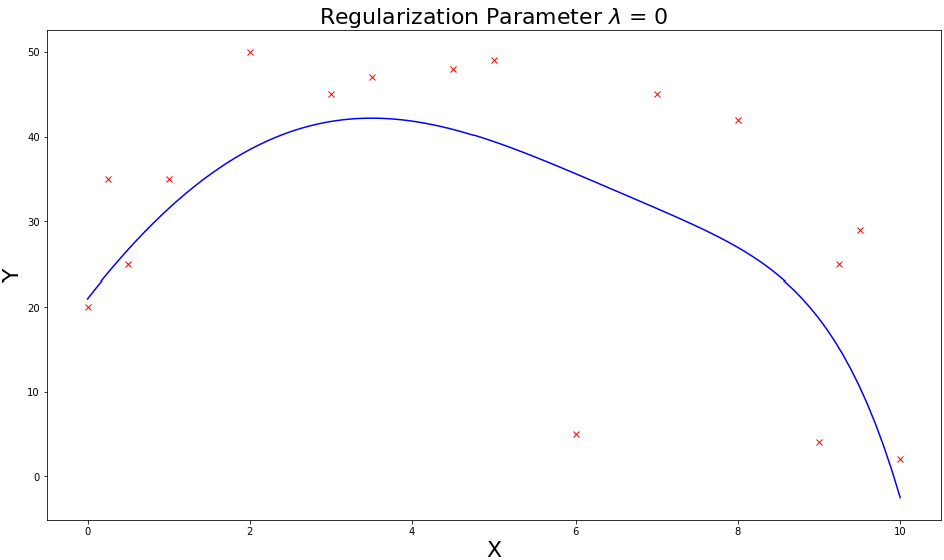
\includegraphics[width=0.8\textwidth]
            {fig_1.png}
            \caption{$\lambda = 0$}
            \label{fig:1}
		\end{figure}    
		
		\begin{figure}[h]
			\centering
			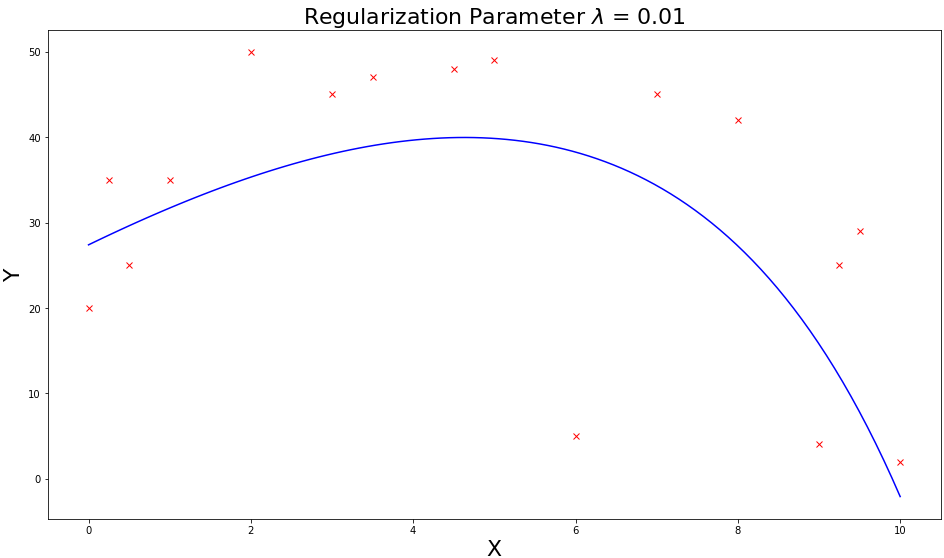
\includegraphics[width=0.8\textwidth]
            {fig_2.png}
            \caption{$\lambda = 0.01$}
            \label{fig:2}
		\end{figure}    
        
\end{document}